\documentclass{beamer}
\usepackage[utf8]{inputenc}
\usepackage{graphicx}

\newtheorem{definicion}{Definición}
\newtheorem{ejemplo}{Ejemplo}

%%%%%%%%%%%%%%%%%%%%%%%%%%%%%%%%%%%%%%%%%%%%%%%%%%%%%%%%%%%%%%%%%%%%%%%%%%%%%%%
\title[Series numéricas]{Series numericas: Función sin(x)}
\author[Jorge, Elizabeth, Yessica]{Jorge Antonio Herrera Alonso, Elizabeth Hernández Martín, Yessica Sabrina Gómez Buso}
\date[12-05-2014]{12 de mayo de 2014}
%%%%%%%%%%%%%%%%%%%%%%%%%%%%%%%%%%%%%%%%%%%%%%%%%%%%%%%%%%%%%%%%%%%%%%%%%%%%%%%
\usetheme{Madrid}
%\usetheme{Antibes}
%\usetheme{tree}
%\usetheme{classic}

%%%%%%%%%%%%%%%%%%%%%%%%%%%%%%%%%%%%%%%%%%%%%%%%%%%%%%%%%%%%%%%%%%%%%%%%%%%%%%%
\definecolor{pantone254}{RGB}{122,59,122}
\definecolor{pantone3015}{RGB}{0,88,147}
\definecolor{pantone432}{RGB}{56,61,66}
\setbeamercolor*{palette primary}{use=structure, fg=white,bg=pantone254}
\setbeamercolor*{palette secondary}{use=structure, fg=white,bg=pantone3015}
\setbeamercolor*{palette tertiary}{use=structure, fg=white,bg=pantone432}
%%%%%%%%%%%%%%%%%%%%%%%%%%%%%%%%%%%%%%%%%%%%%%%%%%%%%%%%%%%%%%%%%%%%%%%%%%%%%%%

\begin{document}
  
%++++++++++++++++++++++++++++++++++++++++++++++++++++++++++++++++++++++++++++++  
\begin{frame}

  \titlepage

  \begin{small}
    \begin{center}
     Facultad de Matemáticas \\
     Universidad de La Laguna
    \end{center}
  \end{small}

\end{frame}
%++++++++++++++++++++++++++++++++++++++++++++++++++++++++++++++++++++++++++++++  

%++++++++++++++++++++++++++++++++++++++++++++++++++++++++++++++++++++++++++++++  
\begin{frame}
  \frametitle{Índice}  
  \tableofcontents[pausesections]
\end{frame}
%++++++++++++++++++++++++++++++++++++++++++++++++++++++++++++++++++++++++++++++  

 

\section{Motivación y objetivos}
\begin{frame}
\frametitle{Motivación y objetivos}
\begin{block}{Motivación}
Aprendizaje orientado al lenguaje de programación $Python$, el procesador de texto $LaTEX$ y el creador de presentaciones $Beamer$.
\end{block}
\begin{block}{Objetivos}
  \begin{itemize}
  \item {\bf Objetivo principal:} Implementación de $Python$ del método de Taylor.\pause
  \item {\bf Objetivo específico:} Aproximación de una función mediante el método de Taylor.
  \end{itemize}
\end{block}


\end{frame}
%++++++++++++++++++++++++++++++++++++++++++++++++++++++++++++++++++++++++++++++  
\section{Fundamentos teóricos}

\subsection{Teorema de Taylor}
%++++++++++++++++++++++++++++++++++++++++++++++++++++++++++++++++++++++++++++++

\begin{frame}
\frametitle{Teorema de Taylor}

\begin{block}{Teorema de Taylor:}
El Teorema de Taylor permite obtener aproximaciones polinómicas de una función en un entorno de cierto punto en que la función sea diferenciable. 
Además el teorema permite acotar el error obtenido mediante dicha estimación. 
\end{block}
\begin{definicion}
Sea I un intervalo, $c$ un punto de I, $f$ una función definida en I. Supongamos que $f$ es derivable en todos los puntos hasta el orden
$n-1$ y que existe $f ^ n (c)$. Entonces:
\tiny{
\[\quad \lim_{x\to c} \frac{1}{(x-c)^n} [ f(x) - f(c) - f '(c) (x-c) - \frac{1}{2!} f '' (c) (x-c) ^ 2 - ...- \frac{1}{n!} f ^ n(c) (x-c) ^ n ] = \text 0\]
}
\end{definicion}

\end{frame}

%++++++++++++++++++++++++++++++++++++++++++++++++++++++++++++++++++++++++++++

\subsection{Polinomio de Taylor}

%++++++++++++++++++++++++++++++++++++++++++++++++++++++++++++++++++++++++++++
\begin{frame}
\frametitle{Polinomio de Taylor}
\begin{definicion}
Dada una función $f$ derivable $n$ veces en un punto $c$. se llama polinomio de Taylor en $c$ de orden $n$ al
polinomio:
\end{definicion}
\begin{block}{ }
	    $f(x) = f(c) + f '(c) (x-c) + \frac{1}{2!} f '' (c) (x-c) ^ 2 + ...... + \frac{1}{n!} f ^ n(c) (x-c) ^ n$
\end{block}
\end{frame}

%+++++++++++++++++++++++++++++++++++++++++++++++++++++++++++++++++++++++++++++
\section{Procedimiento experimental}

\subsection{Descripción de los experimentos}
%++++++++++++++++++++++++++++++++++++++++++++++++++++++++++++++++++++++++++++++  
\begin{frame}
\frametitle{Descripción de los experimentos}
\begin{block}{Descripción:}
  \begin{enumerate}
    \item Realización de varios códigos en Lenguaje $Python$. \pause
    \item Repetición de la ejecución del código. \pause
    \item Aproximación $f(x) =sin(x)$ mediante el método de Taylor. \pause
    \item Error estimado. \pause
    \item Tiempo CPU. 
  \end{enumerate}
\end{block}
\end{frame}
%++++++++++++++++++++++++++++++++++++++++++++++++++++++++++++++++++++++++++++++  

\subsection{Descripción del material}

%++++++++++++++++++++++++++++++++++++++++++++++++++++++++++++++++++++++++++++++  
\begin{frame}
\frametitle{Descripción del material}


  El material requerido para la realización del trabajo ha sido una computadora.


\begin{block}{Carácterísticas de la computadora:}
  \begin{itemize}
    \item  CPU type: Intel(R) Core(TM) i3-2328M CPU @ 2.50GHz \pause
    \item  vendor ID	GenuineIntel\pause
    \item  CPU speed	1200.000Hz\pause
    \item <4->   cache size	2048 KB
  \end{itemize}
\end{block}

\end{frame}
%++++++++++++++++++++++++++++++++++++++++++++++++++++++++++++++++++++++++++++++  

\subsection{Análisis de los resultados}

%++++++++++++++++++++++++++++++++++++++++++++++++++++++++++++++++++++++++++++++  
\begin{frame}
\frametitle{Análisis de los resultados}

\begin{block}{Experimentos realizados:}
  \begin{enumerate}
    \item
     Grado del polinomio y punto $c$, fijos. El punto $x$ cambia. 
      \pause
     
    \item
    Grado del polinomio y punto $x$, fijos. El punto $c$ cambia.
      \pause

    \item
    Grado del polinomio toma el valor 10. Punto $c$ y punto $x$, igual que el experimento 1. 
      \pause
    
    \item
   Grado del polinomio toma el valor de 100. El punto $c$, fijo. El punto $x$ solo varia en las cantidad de cifras decimales. 

  \end{enumerate}
\end{block}

\end{frame}
%++++++++++++++++++++++++++++++++++++++++++++++++++++++++++++++++++++++++++++++  
\section{Algoritmo}
\frametitle{Algoritmo}
\tiny{
\begin{block}{Algoritmo principal:}
\begin{verbatim}

#!/src/bin/python
#!encoding: UTF-8
import math 
from sympy import *
import modulo
import time
import numpy as np 
import matplotlib.pyplot as mp

numero = int(raw_input("Introduzca el grado que desea que tenga el Polinomio de Taylor: "))
centro = float(raw_input("Introduzca el punto central donde desea que se evalue el Polinomio de Taylor: "))
x = float(raw_input("Introduzca el punto x donde desea evaluar el Polinomio de Taylor: "))

modulo.taylor1(x, numero, centro)
y1 = np.linspace(-np.pi, np.pi, 256, endpoint=True)
y1 = np.arange(-8,8,0.1)
y2 = np.sin(y1)
  
mp.plot(y1,y2, color = 'blue',linewidth=2.5, linestyle="-", label="seno")  
mp.legend(loc=0) 

# Para poner el simbolo pi en el eje x se usa LaTeX.
mp.xticks([-2*np.pi, -3*np.pi/2, -np.pi, -np.pi/2, 0, np.pi/2, np.pi, 3*np.pi/2, 2*np.pi],
[r'$2\pi$',r'$-\frac{3\pi}{2}$',r'$-\pi$',r'$-\frac{\pi}{2}$',r'$0$',r'$+\frac{\pi}{2}$',r'$+\pi$',
r'$\frac{3\pi}{2}$',r'$2\pi$'])  

mp.title("Representacion grafica")         
 
mp.savefig('grafico.png',dpi = 100)

mp.show()
\end{verbatim}
\end{block}
\begin{block}{Algoritmo del módulo}
\begin{verbatim}
/#!/src/bin/python
import math
from sympy import *
import time
def factorial(numero):
  factorial = 1
  while(numero > 1):
    factorial = factorial * numero
    numero = numero - 1
  return factorial

def taylor1(x, numero, centro):
  inicio = time.time()
  c = Symbol('c')
  f = sin(c)
  func = f.evalf(subs={c: centro})
  suma = func
  for i in range (1,numero + 1):
    f_i = diff(f, c)
    v = f_i.evalf(subs={c: centro})
    s= (v / factorial(i)) * ((x - centro) ** i)    
    suma = suma + s
    f = f_i
  error = func - suma
  print 'El valor de la funcion original sin(%f) es igual a %f ' % (centro, func)
  print 'El Polinomio de Taylor de grado n=%d en el punto centro c=%f 
  evaluada en el punto x=%f es igual a %f' % (numero, centro, x, suma)
  print 'El Error de la funcion original con el Polinomio de Taylor es: error=%f' % error
  l=[numero, centro, x, suma, error]
  f = open("Taylor.tex", 'a')
\end{verbatim}
\end{block}
\begin{block}{ }
\begin{verbatim}
  f.write('Grado del Polinomio (n) Punto Central (c)  Punto de Evaluacion (x)  
  Aproximacion
  Error Tiempo CPU \n ')
  fin = time.time()
  tiempo_total = fin - inicio
  l=l+[tiempo_total]
  f.write(str(l))
  f.write("\n")
  f.close()
  f=open("Taylor.tex","r")
  print(f.read())
  f.close()
  return taylor1
\end{verbatim}
\end{block}
}
%++++++++++++++++++++++++++++++++++++++++++++++++++++++++++++++++++++++++++++++
\section{Gráfica}
\frametitle{Gráfica}
\begin{block}{Gráfica}
\begin{center}
\begin{figure}[!th]
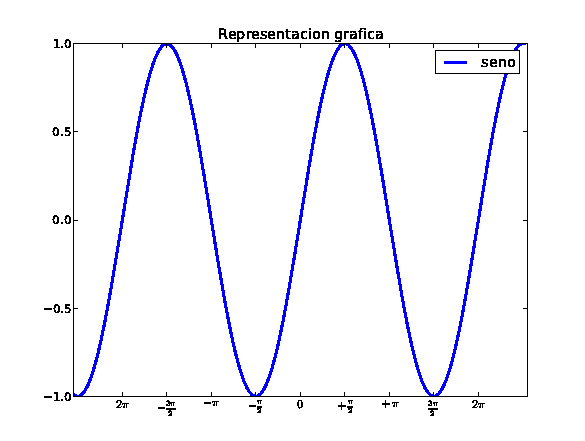
\includegraphics[width=0.75\textwidth]{images/grafica.png}
\caption{Gráfica de la función original}

\end{figure}
\end{center}
\end{block}
%++++++++++++++++++++++++++++++++++++++++++++++++++++++++++++++++++++++++++++++

\section{Tablas}

\subsection{Experimentos 1 y 2}
\begin{frame}
\frametitle{Tablas}

\begin{table}[!ht]
\begin{center}
\begin{tabular}{|l|c|c|c|c|c|}
\hline
Grado  & Punto c & Punto de Evaluacion & Aproximacion       & Error             & Tiempo CPU           \\ \hline
4      &   0.0   &    1                & 0.833333           & -0.833333         & 0.007406949996948242 \\ \hline
6      &   10    &    5                & 12.4605618963148   & -13.0045830072041 & 0.009202957153320312 \\ \hline
10     &   10    &    10               & -0.544021110889370 & 0                 & 0.010988950729370117  \\ \hline
\end{tabular}
\end{center}
\caption{Tabla de datos obtenidos experimentalmente}
\label{tab}
\end{table}

\end{frame}

\subsection{Experimentos 3 y 4}
\begin{frame}
\frametitle{Tablas}

\begin{table}[!ht]

\begin{tabular}{|l|c|c|c|c|c|}
\hline
Grado  & Punto c & Punto x & Aproximacion       & Error             & Tiempo CPU            \\ \hline
10     & 10.0    & -10.0   & 2226636.13194962   & -2226636.67597073 & 0.012552976608276367  \\ \hline
10     & 10.0    &  -5.0   & 124685.902313545   & -124686.446334656 & 0.011905908584594727  \\ \hline
10     & 10.0    &   0.0   & 1920.68755204547   & -1921.23157315635 & 0.011946916580200195  \\ \hline
10     & 10.0    &   5.0   & 0.163743739637233  & 0.707764850526603 & 0.08893513679504395   \\ \hline
10     & 10.0    &   9.0   & 0.412118507257685  &-0.956139618147055 & 0.014183998107910156  \\ \hline
10     & 10.0    &   9.9   & -0.457535893775321 &0.0864852171140484 & 0.012012958526611328  \\ \hline
10     & 10.0    &  10.0   & -0.544021110889370 &        0          & 0.014500856399536133  \\ \hline
\end{tabular}

\caption{Tabla de datos obtenidos. Experimento 3}
\label{tab}
\end{table}


\begin{table}[!ht]

\begin{tabular}{|l|c|c|c|c|c|}
\hline
Grado  & Punto c & Punto x & Aproximacion       & Error             & Tiempo CPU            \\ \hline
100    & -1.0    &-0.99999 &-0.8414655817427645 &-5.40306513208133e & 0.06290507316589355   \\ \hline
100    & -1.0    & -0.9    & -0.783326909627484 &-0.0581440751804130& 0.06340909004211426   \\ \hline

\end{tabular}

\caption{Tabla de datos obtenidos. Experimento 4}
\label{tab}
\end{table}



\end{frame}
%++++++++++++++++++++++++++++++++++++++++++++++++++++++++++++++++++++++++++++++  
\section{Bibliografía}
%++++++++++++++++++++++++++++++++++++++++++++++++++++++++++++++++++++++++++++++  
\begin{frame}
  \frametitle{Bibliografía}

  \begin{thebibliography}{10}

    \beamertemplatebookbibitems
    \bibitem[Tutorial Beamer]{guia}  
    Turorial Beamer. 

    \beamertemplatebookbibitems
    \bibitem[Apuntes de anális I]{latex} 
    Apuntes de análisis I.
    
    \beamertemplatebookbibitems
    \bibitem[Tutorial LaTex]{plan}  
    Comandos latex - Páginas - Fórmulas - Bibliografías. 

   

  \end{thebibliography}
\end{frame}

%++++++++++++++++++++++++++++++++++++++++++++++++++++++++++++++++++++++++++++++  
\end{document}
